\begin{figure}[ht]
    \centering
    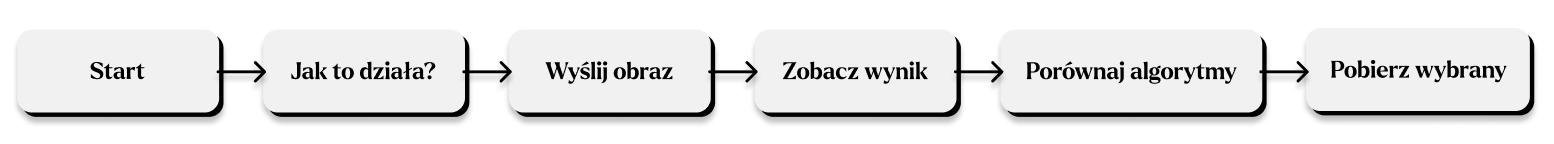
\includegraphics[width=\linewidth]{Rozdziały/06.Aplikacja/Obrazy/user-flow.png}  
    \caption{Diagram przepływu użytkownika}
    \label{fig:image82}
\end{figure}

TODO: Usuń diagram przepływu

\section{Implementacja aplikacji}

Po wyborze stosu technologicznego kolejnym krokiem jest skupienie się na implementacji rozwiązań. W tym rozdziale opiszę jakie decyzje podjąłem przy pisaniu kodu aplikacji, jak wygląda jej struktura i jakie problemy napotkałem podczas implementacji.

\subsection*{Struktura aplikacji}

Aplikacja składa się z dwóch części - Frontendu i Backendu. Przy tworzeniu takiego projektu warto zadbać o to, żeby każda część była od siebie niezależna i żeby komunikacja między nimi była jak najmniej skomplikowana.

W tym miejscu wracamy do diagramu przepływu użytkownika [Rys \ref{fig:image82}], jak na nim widać użytkownik nie może wykonać zbyt wiele akcji, struktura aplikacji jest liniowa. Na podstawie diagramu przepływu użytkownika można stworzyć schemat blokowy aplikacji [Rys \ref{fig:image87}], który pozwoli zrozumieć zachowanie programu.

\begin{figure}[H]
    \centering
    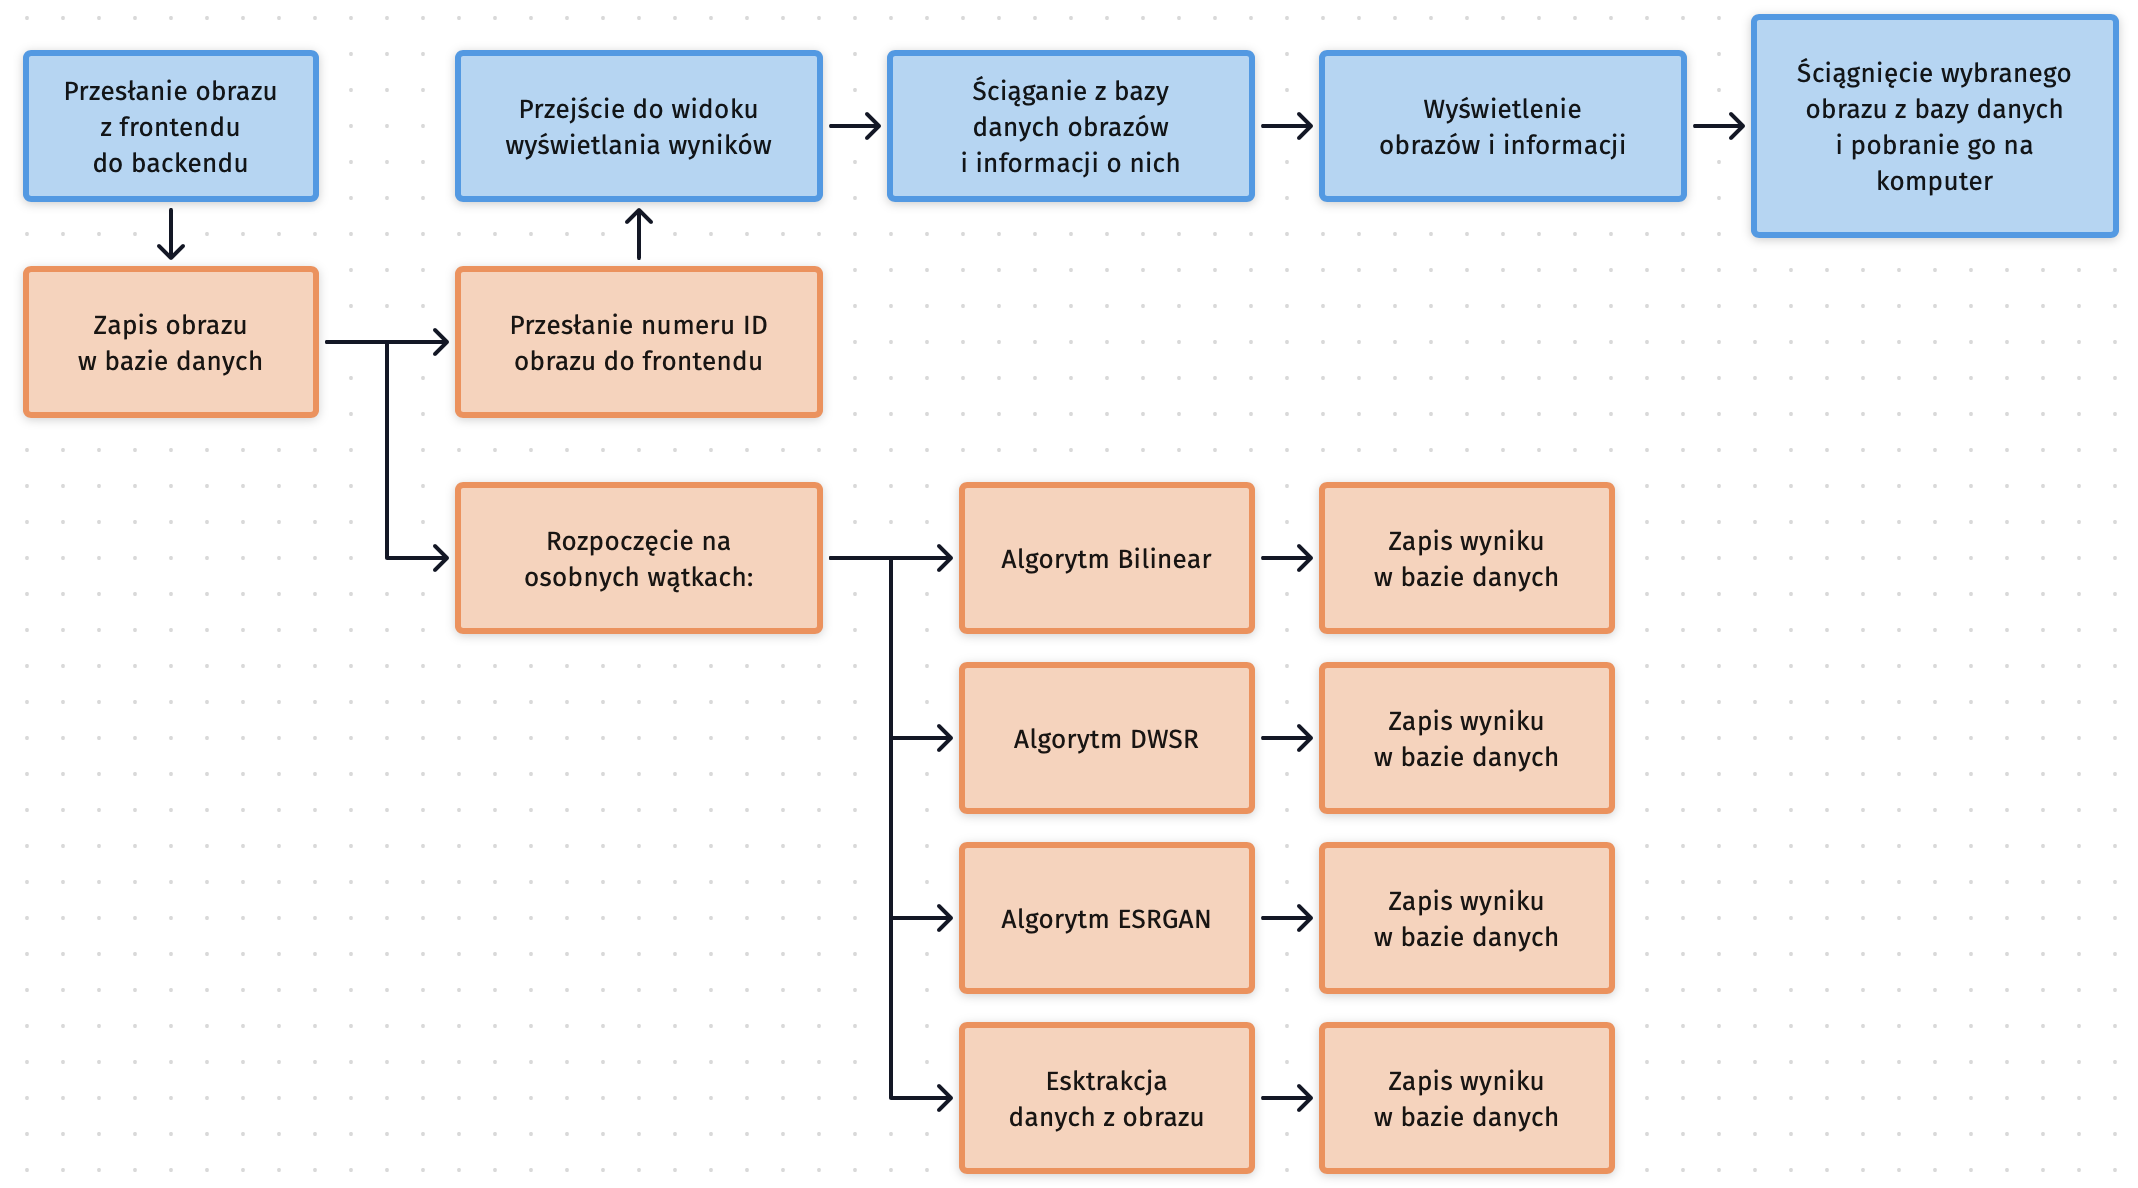
\includegraphics[width=\linewidth]{Rozdziały/06.Aplikacja/Obrazy/mechanizm_aplikacji.png}  
    \caption{Schemat blokowy aplikacji (kolor niebieski - Frontend, pomarańczowy - Backend)}
    \label{fig:image87}
\end{figure}

W pierwszej kolejności użytkownik wysyła obraz do serwera Backend, który zapisuje go w bazie danych. Następnie serwer zleca wykonanie algorytmów na osobnych wątkach, o czym opowiem w dalszej części rozdziału [\ref{sec:implementation-s-r}]. Gdy algorytmy rozpoczną pracę, serwer zwraca do Frontendu informację o tym że operacja zapisu się powiodła i podaje numer ID obrazu. 

Frontend zmienia widok na ten z wynikami i wysyła zapytanie do Backendu o obraz oryginalny i przetworzone. Następnie jeśli serwer zwróci obrazy, Frontend je wyświetla. W przeciwnym wypadku próbuje je pozyskać ponownie aż do skutku. Dzieje się tak, dlatego że zadanie super-rozdzielczości jest czasochłonne i czasem może zająć kilka sekund a w innych wypadkach nawet kilka minut, wszystko w zależności od rozdzielczości obrazów. W tym czasie użytkownik może porównywać uzyskane wyniki i wybrać najlepszy. 

Gdy użytkownik wybierze obraz, może go pobrać na swój komputer. Wtedy Frontend wysyła zapytanie do serwera o obraz w pełnej rozdzielczości, a serwer zwraca obraz wraz z nagłówkiem \textit{Content-Disposition: attachment} co powoduje, że przeglądarka automatycznie pobiera obraz na dysk użytkownika.

\subsubsection*{Architektura bazy danych}

Baza danych w aplikacji jest bardzo prosta, przy przesłaniu każdego zdjęcia w bazie tworzone jest pole Image, które przechowuje informacje o obrazie oraz jego przetworzonych wersjach. W tabeli \ref{tab:image_model} przedstawiam jedyną tabelę w bazie danych, która przechowuje informacje o obrazach.

\begin{table}[ht]
    \centering
    \renewcommand{\arraystretch}{1.5} % Increase row height by 1.25 times
    \begin{tabular}{|l|l|p{8cm}|}
    \hline
    \multicolumn{3}{|c|}{\textbf{Image}}                                                        \\ \hline
    \textbf{Pole}       & \textbf{Typ}          & \textbf{Opis}                                 \\ \hline
    image               & ImageField            & Przesłany obraz.                              \\ \hline
    bilinear\_image     & ImageField            & Obraz powiększony algorytmem Bilinear.        \\ \hline
    dwsr\_image         & ImageField            & Obraz powiększony algorytmem DWSR.            \\ \hline
    esrgan\_image       & ImageField            & Obraz powiększony algorytmem ESRGAN.          \\ \hline
    original\_height    & PositiveIntegerField  & Wysokość oryginalnego obrazu.                 \\ \hline
    original\_width     & PositiveIntegerField  & Szerokość oryginalnego obrazu.                \\ \hline
    dominant\_colors    & TextField             & Pole tekstowe z listą dominujących kolorów.   \\ \hline
    \end{tabular}
    \caption{Struktura bazy danych - Image.}
    \label{tab:image_model}
\end{table}

Jak widać w bazie danych przechowywane są obrazy w formacie \textit{ImageField}, który jest dostarczany przez bibliotekę Django. Jest to pole, które przechowuje ścieżkę do pliku na dysku serwera. Zapisujemy również informacje o oryginalnych wymiarach obrazu, które są wyświetlane użytkownikowi przez Frontend. 

Dodatkowo w bazie danych przechowujemy listę dominujących kolorów, które są wykrywane przez algorytm K-średnie \textit{K-means}, o którym opowiem w kolejnym rozdziale [\ref{sec:implementation-s-r}]. Jest to lista kolorów w formacie HEX, które wykorzystuje Frontend do wyświetlenia kolorowych gradientów tła.


\newpage
\section{Integracja algorytmów super-rozdzielczości} \label{sec:implementation-s-r}




\begin{lstlisting}[language=Python, caption=Obsługa zapisu i przetwarzania obrazów (Django).]
    def upload_image(request):
    try:
        form = Image(image=request.FILES['image'])
        form.save()

        input_image_path = form.image.path
        
        thread1 = threading.Thread(target = run_bilinear, 
                                   args = (input_image_path, 4, form))
        thread2 = threading.Thread(target = run_dwsr, 
                                   args = (input_image_path, 4, form))
        thread3 = threading.Thread(target = run_esrgan, 
                                   args = (input_image_path, form))
        thread4 = threading.Thread(target = extract_image_info, 
                                   args = (input_image_path, form))

        thread1.start()
        thread2.start()
        thread3.start()
        thread4.start()

        image = Image.objects.latest('id')  # Gets the latest entry

        return JsonResponse({'message': 'Image uploaded, processing started', 
                             'image_id': image.id})

    except Exception as e:
        return JsonResponse({'error': str(e)}, status=400)
\end{lstlisting}





\section{Testowanie aplikacji}




\section{Wdrożenie i utrzymanie aplikacji}

Omówienie procesu wdrożenia gotowej aplikacji oraz planów dotyczących jej przyszłego utrzymania i aktualizacji.



\section{Plany na przyszłość} \label{sec:plans}

Opis błędów, rzeczy do poprawy w aplikacji. Omówienie jakie są plany rozbudowy aplikacji.

Przyciski nawigacji z widoku do widoku